%% =============Chapter 3 starts here===================== 

\chapter{Where's Waldo: Looking closely at a Lineup} \label{ch:waldo}
\vspace{-0.8cm}
\large{Niladri Roy Chowdhury, Heike Hofmann, Dianne Cook, Mahbubul Majumder, Yifan Zhao}\\ \\
\large{This paper won the Student Paper Award in Section on Statistical Graphics and will be presented in Joint Statistical Meetings 2012. } 

%\maketitle
\vspace{1cm}
\normalsize
 Graphics play a crucial role in statistical analysis and data mining. This paper describes developments to assist the use of graphics for making inferential statements. It examines the lineup protocol described in \citet{buja:2009}  
  developing numerical statistics to measure the quality of the lineup. Distance measures are developed that describe how close the observed data plot is to the null plots, and how close the null plots are to each other. These measures are compared with choices made by human judges, to decide on the best distance measures to use for particular plot types.

\section{Introduction} 
There have been major advances in statistical graphics over the years, for example, systems like \texttt{R} (\cite{r}) provide high quality static graphics, and very recently some access to interactive graphics. But the problem remains that graphics are not widely considered to be a part of inferential statistics. Research by \citet{gelman:2004} and \citet{buja:2009} 
potentially changes this. 

The lineup protocol in \citep{buja:2009} 
places a statistical plot firmly in the hypothesis testing framework. The plot of the data is considered to be a test statistic, and this plot is compared with plots from the appropriate null distribution, producing the lineup. Plots from the null distribution can be generated in many ways, depending on the specification of the null. For parametric testing, data can be simulated from a statistical distribution. For non-parametric testing, other data generating mechanisms may be implied. For example in a lineup using scatterplots, where the null hypothesis is no association between the two variables,  a null generating mechanism is to permute one column of numbers. The marginal distributions of the two variables stay the same while any association between the variables is broken. For more details, see \cite{GOOD05}.

The lineup protocol is analogous to the statistical significance calculations in traditional statistical tests. In hypothesis testing, the observed value of the test statistic is compared with all possible values of its null distribution. If the statistic is extreme on this scale, there is evidence to disbelieve the null hypothesis. With the lineup protocol, for a data plot to be considered to be extreme, a human judge must pick it as different from the other plots in the lineup. 

A major difference is that although the distribution of null plots might be infinite, a human judge can view just a finite number of plots. A lineup will consists of $m$ (typically 20) plots, one of which is the observed data plot, the judge gets to pick whether one plot is different. This finite choice of null plots poses a small wrinkle in the lineup protocol. As Tukey suggested, `there is such a thing as a bad random sample' \citep{fernholz03}:

\begin{quotation}
There [in Tukey's Data Analysis class] I discovered that [...]  a random sample is indeed a ``batch of values'' which ``fail to be utopian'' most of the time.
\end{quotation}

To avoid basing conclusions on artifacts introduced by a `bad' sample, we need to be aware of properties of this set of null plots. In this paper, we develop techniques that help to determine the quality of the lineup. A variety of distance metrics measuring the ``closeness'' of the observed data plot and the null plots, and the null plots with themselves are examined. These are compared to human subject picks in a small experiment.  Describing plots numerically, is something  of an oxymoron, it cannot be done. The purpose is to help determine if a lineup might provide inadequate coverage of the full null distribution, and these measures might help to gain more insight on how the human eyes work in reading statistical graphics. The next section describes the array of distance measures, and further sections describe the scatterplot example, and the process for evaluating the distance measures. 

%Any statistical analysis must include some sreftatistical graphics. For exploratory data analysis, statistical graphics play an invaluable role in model checking and diagnostics. Even though we have established mathematical procedures to obtain various statistics, we need to support the results by also producing the relevant plots. 

%In recent times there have been major advances in statistical graphics. Modern computing systems like R and SAS produce high quality statistical graphics. Buja et al. 2009, following from Gelman 2004, proposed two protocols that allow the testing of discoveries made from statistical graphics.

%In this paper we are interested in the quality of a lineup plot. In visual inference, the actual plot is the test statistic and the lineup plot is the null distribution. Unlike classical inference, the null distribution is represented by the 19 null plots that we obtain randomly from the actual plot assuming that the null hypothesis is true. So the decision of rejection or failure of rejection of the null hypothesis is heavily dependent on these 19 null plots. This induces us to take a closer look at the null plots. For this purpose, we calculate different distance matrices between the null plots and the actual plot to get a measure on how close is each null plot to the actual plot. We also calculate the distance matrices between the null plots to see how close are the null plots to each often. Finally a percentile value is calculated to find how often such a distance appears in a lineup and a z-score of the different distances is calculated to get a measure on the closeness between the null plot and the actual plot and also compare between two different lineups.  

%In this paper we presents results of a human-subject study assessing the performance of the different distance matrices. Section \ref{sec:visual_test} describes the basic idea of the visual inference and also gives the definition of the different distance measures. Section \ref{sec:asso} and Section \ref{user.distance} applies these ideas and uses the definitions to calculate the different distance measures. In Section \ref{results} and Section \ref{sec:conclusions} we outline the setup and present results.

%\section{Visual Statistical Inference and Definitions} \label{sec:visual_test} 

%This section outlines the concepts of visual inference in comparison to the procedures of classical statistical inference and also gives the definition of the different distance measures. 

%Let $\theta$ be a population parameter of interest, with $\theta \in \Theta$, the parameter space. 
%Any null hypothesis $H_0$ then partitions the parameter space into $\Theta_0$ and $\Theta_0^c$, with $H_0: \theta \in \Theta_0$ versus $H_1: \theta \in \Theta_0^c$. 
% In hypothesis testing terminology, the parameter space $\Theta$ of a population parameter $\theta$, can be partitioned into $\Theta_0$ and $\Theta_0^c$. We test $H_0: \theta \in \Theta_0$ versus $H_1: \theta \in \Theta_0^c$.

%\subsection{Visual Statistic} 

%Unlike classical hypothesis testing, the statistic in visual inference is not a single value, but a plot that is appropriately chosen to describe the parameter of interest, $\theta$. When the alternative hypothesis is true, it is expected that the plot of the observed data, the test statistic, will have visible feature(s) consistent with $\theta \in \Theta_0^c$, and that visual artifacts will not distinguish the test statistic as different when $H_1$ is not true.

%\begin{dfn}\label{dfn:lplot}
%A lineup plot is a layout of $m$ visual statistics, consisting of 
%\begin{itemize}\itemsep-3pt
%\item $m-1$ plots simulated from the model specified by $H_0$  (null plots) and 
%\item the test statistic produced by plotting the observed data, possibly arising from $H_1$.
%\end{itemize}
%\end{dfn}

%If $H_1$ is true, the test statistic is expected to be the plot that is most different from the other plots in the lineup plot. A careful visual inspection should reveal the differences in the feature shown by the test statistic under null and alternative hypothesis. {\em If the test statistic cannot be identified} in the lineup, the conclusion is to {\em not reject the null hypothesis.} The $(m-1)$ null plots can be considered to be samples drawn from the sampling distribution of the test statistic assuming that the null hypothesis is true. \\

%Since the lineup plot consists of $m$ plots, the probability of choosing any one of them is $1/m$. Thus we have a type-I error probability of $1/m$.

%\red{the next three paragraphs might be important, but you loose focus - you want to come as fast as possible to the problematic of the paper, e.g.:}
%The lineup plot can be evaluated by one or more individuals. When a single individual identifies the observed graph in the lineup plot we report a $p$-value of at most $1/m$, otherwise the $p$-value is at least $1-\frac 1m$. 
%
%If $N$ individuals evaluate a lineup plot independently, we count the number of successful evaluations as $U \sim \text{Binom} (N,\frac{1}{m})$ and report a  $p$-value of at most $Pr(U \ge u)= \sum_{k \ge u}^N {{N \choose k} (\frac{1}{m})^k(1-\frac 1m)^{(N-k)}}$ where $u$ is the observed number of successful evaluations. %Notice that when $N=1$, this $p$-value is $\frac1m$.  \\ 
%
%
%For two different visual test statistics of the same observed data, the one  is better, in which a specific pattern is more easily distinguishable visually. \\ \\

%\red{Before distance measures are introduced, introduce the problem of why we look at these distances in the context of permutation tests. }
%The difference between a regular permutation test and a graphical test under the line-up protocol, is that we are comparing the observed value of the test statistics (i.e. the plot of the observed data) to a finite sample of the sample distribution.


\section{Distance Measures}\label{defn.distance}

%\blue{The difference between a regular permutation test and a graphical test under the line-up protocol, is that we are comparing the observed value of the test statistics (i.e. the plot of the original data) to a finite sample of the sample distribution. As Tukey suggested, `there is such a thing as a bad random sample' \citet{fernholz03}:
%\begin{quotation}
%There [in Tukey's Data Analysis class] I discovered that [...]  a random sample is indeed a ``batch of values" which ``fail to be utopian" most of the time.
%\end{quotation}
%
%To avoid basing our conclusion on artifacts introduced by a `bad' sample, we need to be aware of properties of this set of null plots. In this paper, we are proposing a set of  distance measures that help us in the evaluation of the goodness of a random sample. It also turns out, that these measures give us also some insight in the perceived difficulty of picking the original plot of the data from a particular line-up. 
%
%\subsection*{Distance Measures}
%}

%\red{The distance measures need some more setting up beforehand. I would actually include a small example of a set of scatterplots that highlights the problematic.}
%
%\red{Another thing that we should discuss on Friday is whether it might be better to call the measures we use norms rather than distances - a distance usually assumes the comparison of two objects, and we implicitly compare against null or identity, which is what a norm does..}

There are different types of distance measures suitable in measuring the distance between the permuted variable and the original variable. In this paper we used six different types of distance measures so that they can identify the different characteristics present in a plot. \\

For all of the distance measures below, let $P$ be a permutation mapping  the set $\{1, 2, ..., n\}$ onto itself. Let further $[P]$ denote the $n \times n$ matrix associated to permutation $P$.

%\blue{For all of the distance measures below, let $P$ be a permutation mapping  the set $\{1, 2, ..., n\}$ onto itself. Let further $[P]$ denote the $n \times n$ matrix associated to permutation $P$.
%}
\begin{itemize}

\item Hamming Distance: The hamming distance $h$ of $P$ is defined as 
\[
h(P) := \sum_{i=1}^n I_{P(i) \neq i},  \text{ where } I_{x} = \left \{ 
\begin{array}{ll}
1 & \text{if } x \text{ is true},\\
0 & \text{otherwise},
\end{array} \right.
\]
i.e. $h(P)$ is a count of the number of fix elements of the function.


%\blue{
%The hamming distance $H$ of $P$ is defined as 
%\[
%H(P) := \sum_{i=1}^n I_{P(i) \neq i},  \text{ where } I_{x} = \left \{ 
%\begin{array}{ll}
%1 & \text{if } x \text{ is true},\\
%0 & \text{otherwise},
%\end{array} \right.
%\]
%i.e. $H(P)$ is a count of the number of fix elements of the function.
% }

%Hamming distance between two equal length strings is the number of positions at which the corresponding symbols are different. 

This distance matrix measures the distance between the permutation matrix and the identity and does not depend on the actual values of the variables $X$ and $Y$. 


%\blue{let $X$ be a continuous variable. The Euclidean Distance under permutation is then defined as 
%%\red{we need a good short-cut for this distance}
%\[
%d^2_P(X) := || X - [P]X||^2 = \sum_{i=1}^n (X_i - X_{P(i)})^2.
%\]
%}


\item Euclidean Distance of actual values: 
Let $Y$ be a continuous variable. The Euclidean Distance under permutation is then defined as 
%\red{we need a good short-cut for this distance}
\[
d^2_V(X) := || Y - [P]Y||^2 = \sum_{i=1}^n (Y_i - Y_{P(i)})^2.
\]





%Euclidean Distance between two equal length strings measure the distance between the permuted values of one variable and the original continuous variable while the other variable, either continuous or categorical, remains unaltered. This distance matrix takes into  account the actual values of the variable that is permuted and does not depend on the values of the other variable. 

\item Binned Distance:
%\red{write out mathematically, include all definitions - i.e. C(X,Y) needs to be defined - have a look at the grammar of graphics}
Let $X$ and $Y$ be two continuous variables. Let $X$ be divided into $p$ bins and $Y$ divided into $q$ bins. $(i,j)$-th cell represents the $j$-th bin of $Y$ corresponding to the $i$-th bin of $X$. Let $C(X,Y)$ be defined as a $p \times q$ matrix. Each $(i,j)$-th element of the matrix represents the number of points falling in the $(i,j)$-th cell, where $i = 1, \dots, p$ , $j = 1, \dots, q$.
The Binned distance under permutation is then defined as
\begin{eqnarray*}
b^2_P(X) &:=& ||C(X,Y) - C(X,[P]Y)||^2 \\ &=& \sum_{i=1}^p \sum_{j=1}^q (C_{X_i,Y_j} - C_{X_i,P(Y)_j})^2.
\end{eqnarray*}

The usual convention is to take the number of bins equal to the square root of the number of observations. So we take $p = q = \lceil{\sqrt{n}} \rceil$ for $n \leq 100$ and $p = q = 10$ for $n > 100$ where $\lceil{x} \rceil$ is the smallest integer greater than or equal to $x$. \\

Binned distance is highly susceptible to small differences in values and depends on the number of bins as well as exact cut-offs. This is particularly problematic for small number of points. As a remedy to that, we are considering Weighted bin distance next, which is based on the density rather than point frequency. For large number of points the weighted binning is computationally too intensive, in which case we will make use of the unweighted  binned distance.
%\red{careful: $C(X,[P]Y)$ is not the same as $C_{i,P(j)}$. $C_{i,j}$ is the count for points falling into cell $i,j$ - it's not enough to permute the grid counts, we need to get the grid counts of the permuted variable. Introduce $C$ as a function of $X$ and $Y$ ....}

% To calculate this distance, we form a $p \times q$ grid between the two continuous variable and count the number of points falling to each grid. Then we permute one continuous variable keeping the other variable unchanged and repeat the above procedure. The euclidean distance between the counts for the original and permuted data gives an measure of the binned distance. Binned distance takes into account both the variables but only one of the variables is permuted. Binned distance considers only the count for each respective bin and puts no weight on the counts of the neighboring bin.

\item Weighted Bin Distance: Using the same setup of the binned distance, the weighted bin distance under permutation is defined as 
\begin{eqnarray*}
w_P^2(X) &:=&||W(X,Y) - W(X,[P]Y))||^2 \\ &=& \sum_{i=1}^n (W_{X_{i},Y_i} - W_{X_i,P(Y)_i})^2 , 
\end{eqnarray*}
where $W_{X_i,Y_i}$ denotes the joint (empirical) density of $X$, $Y$ at location $(X_i, Y_i)$. See Figure \ref{wbdist} for a comparison of weighted and unweighted binned distance at the example of 20  points.
%The weighted bin distance is an improvement to the bin distance where a weight is provided to the counts of the neighboring bins. The weight is done by doing a kernel density estimation of the different bins.

%\green{I wrote something down here but I am not sure if this works.}

\begin{figure}[hbt]
%\begin{figurehere}
   \centering
       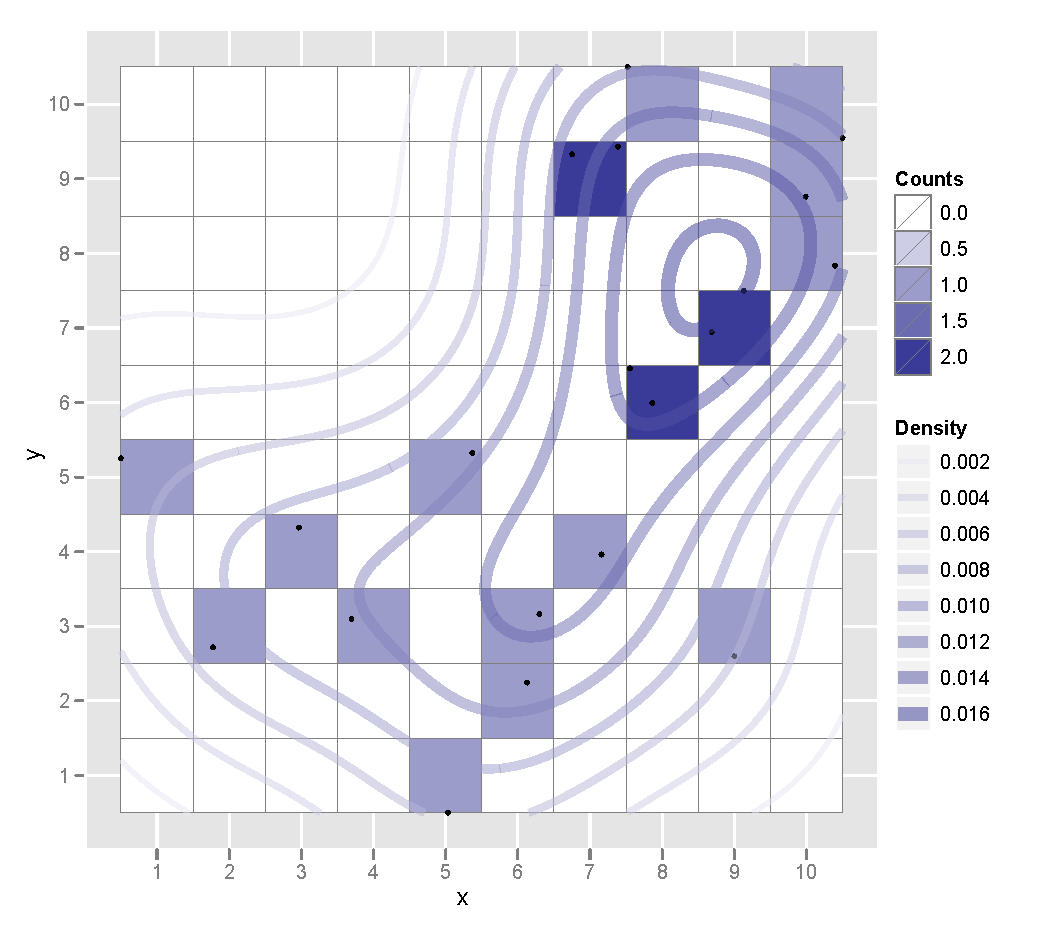
\includegraphics[width=3.3in]{wbdist.pdf}
	\vspace{-.2in}
       \caption{Scatterplot of 20 points in $X$ and $Y$ with a weak positive association. The colored tiles show binned frequencies, the contour lines show two-dimensional density.}
       \label{wbdist}
\end{figure}
\end{itemize}

The remaining distance measures are different from the ones above, in that they are used to directly draw inference on a linear association between variables $X$ and $Y$, whereas the other ones were not specifically tailored to this purpose.

%\blue{The remaining distance measures are different from the ones above, in that they are used to directly draw inference on a linear association between variables $X$ and $Y$, whereas the other ones were not specifically tailored to this purpose.}

\begin{itemize}
\item $t$ statistic: In this paper we used the test statistic of a t-test based on the correlation coefficient $r$ where $$t =\frac{r \sqrt{n - 2}}{\sqrt{1 - r^2}}$$ where $n$ is the number of observations in $X$ or $Y$. This is the only measure that makes a distributional assumption that the ($X$,$Y$) follows approximately a bivariate Normal distribution. Hence the $t$-statistic follows a t distribution with ($n$ - 2) degrees of freedom.
%\red{use either upper case or lower case $T$, not both. }
%The first one was used when one variable is continuous and the other is categorical while the other is used when both the variables are continuous.  

%\item Wilcoxon Rank Sum Test statistic: This is a nonparametric test statistic for assessing whether one of the two samples of independent observations tend to have larger values than the other. This is also used when one variable is continuous and the other is categorical.  

\item Spearman's rank correlation $\rho$ : $\rho$ is a nonparametric alternative to the correlation coefficient with Kendall's $\tau$. $X$ and $Y$ are converted into the ranks $x$ and $y$. Assuming there are no ties in the data, the differences $d_i=x_i - y_i$ between the ranks of each observation between the two variables are calculated and $\rho$ is given as $$\rho = 1 - \frac{6\sum_{i=1}^n d_i^2}{n(n^2 - 1)}$$ The Spearman's rank correlation is a better measure of correlation than the Pearson's rank correlation if the data contains some outliers. Kendall's $\tau$ is computationally intensive.
% - the naive implementation is $O(n^2)$, but it can be reduced to $O(n \log n)$, which is equivalent to sorting.}
%takes huge time \red{could you be more specific - is it $O(n^2)$? - I think it can be brought down to $O(n \log n)$} \green{I think I used 2 for loops. So it should be $O(n^2)$. But I am not sure if it can be brought down to $O(n \log n)$}to calculate for an averaged size sample. 
So in this paper we considered $\rho$ as the only nonparametric measure.
%\red{which one of the statistics do you refer to?} 
%\red{give a mathematical definition of $\rho$}
$\rho$ uses both the variables. 

\end{itemize}

%\section{Inference for difference of two groups} \label{sec:diff}
%
%Consider a dataset with one variable which is essentially continuous. This variable is divided into two groups. Let us call these two groups as Group A and Group B. We can look this dataset as a dataset consisting of two variables, one of which is a continuous variable and the other is a categorical variable with two levels. Now we want to know whether the values of the continuous variable in Group B are generally higher than the values of the continuous variable in Group A. To test this we generate a dot-plot with the two groups represented with two different colors. If the values of the continuous variable for Group B are higher than that for Group A, the dot-plot shows a vertical displacement between the two colored groups. \\
%A lineup including this test statistic is shown in Figure \ref{lineup_dot}. The 19 null plots are generated by permuting the categorical variable while the continuous variable remained unaltered. The test statistic, the plot containing the observed data, is placed randomly among these null plots. If the test statistic is identifiable, the null hypothesis is rejected with a $p$-value of at most 0.05. 
%
%\begin{figure}[hbt]
%%\begin{figurehere}
%   \centering
%       \scalebox{0.5}{\includegraphics{dotplot7.pdf}}
%       \caption{Lineup Plot (m = 20) for testing whether the Group B is generally larger than Group A. The 19 null plots are obtained by permuting the groups while keeping the continuous variable unaltered. Can you identify the observed plot?}
%       \label{lineup_dot}
%\end{figure}
%
%We calculated the distance matrices defined in Section \ref{sec:visual_test} between each of the null plots and the actual plots. Since some of the distance matrices requires both the variables to be continuous , we calculate only the Hamming, the Eucildean, the t-statistic and the Wilcoxon Rank Sum test statistic. In this case the hamming distance is calculated by permuting the categorical variable and looking at the number of positions at which the groups are different between the observed data and the permuted data. We also calculated the percentile value based on each distance matrices for each of the null plots by finding how many distances smaller than the one obtained for the null plot can we get if we generate 10,000 distances corresponding to the 10,000 permutations of the observed data. We repeat the above procedure for all the null plots and all the distances. This tells us how likely it is to observe a particular null plot when you have the observed data. Figure \ref{emp_eucl} shows the empirical distribution of the Euclidean distances for the observed data. We save the different distances for all the null plots ordered according to the smallest percentile value. Table \ref{dot_table} shows the four different distances and the percentile values obtained based on each distance.
%
%\begin{figure}[hbt]
%%\begin{figurehere}
%   \centering
%       \scalebox{0.45}{\includegraphics{emp_eucl.pdf}}
%       \caption{Plot showing the empirical distribution of the Euclidean Distance. The vertical red line shows the euclidean distance between the observed data to itself which is 0. The blue vertical lines shows the euclidean distance between Plot 14 and Plot 6 from the observed data.   }
%       \label{emp_eucl}
%\end{figure}
%
%\begin{table*}[hbt]
%\caption{Table showing the different distance matrices and the percentile values of each distance \red{always align numbers along the decimal point. get rid of all vertical lines . stubs, i.e. Distance names need to go in the first line of their set of corresponding rows.}}  % title name of the table
%\centering  % centering table
%\begin{tabular}{l r rrrr}  % creating 10 columns
%\hline\hline                       % inserting double-line
%Distance & PlotNo &\multicolumn{4}{c}{Percentile Value} \\ [0.5ex]   
%\hline  \hline
% & & Hamming & Euclidean & t statistic & Wilkoxon Rank Sum   \\     [0.5ex]
%\hline
%%% Entering 4th row
% Hamming  & 6 & $0.42$ & $0.58$ & $0.02$ & $0.06$  \\[-0.5ex]
%& 14 & $ 0.42$ & $0.02$ & $0.01$ & $0.01$  \\[-0.5ex]
% & 13 & $7.20$ & $18.35$ & $7.19$ & $6.98$  \\[-0.5ex]
% & 16 & $7.20$ & $3.56$ & $3.38$ & $3.08$  \\[1ex]
%\hline
%%% Entering 4th row
%Euclidean & 14 & $0.42$ & $0.02$ & $0.01$ & $0.01$  \\[-0.5ex]
%& 6 & $0.42$ & $0.58$ & $0.02$ & $0.06$  \\[-0.5ex]
% & 16 & $7.20$ & $3.56$ & $3.38$ & $3.08$  \\[-0.5ex]
%& 9 & $36.82$ & $10.69$ & $10.13$ & $8.34$  \\[1ex]
%\hline
%%% Entering 5th row
%t statistic & 14 & $0.42$ & $0.02$ & $0.01$ & $0.01$  \\[-0.5ex]
% & 6 & $0.42$ & $0.58$ & $0.02$ & $0.06$  \\[-0.5ex]
% & 16 & $7.20$ & $3.56$ & $3.38$ & $3.08$  \\[-0.5ex]
%& 5 & $36.82$ & $15.82$ & $7.11$ & $6.98$  \\[1ex]
%% [1ex] adds vertical space
%\hline
% Wilcoxon & 14 & $0.42$ & $0.02$ & $0.01$ & $0.01$  \\[-0.5ex]
%& 6 & $0.42$ & $0.58$ & $0.02$ & $0.06$  \\[-0.5ex]
% & 16 & $7.20$ & $3.56$ & $3.38$ & $3.08$  \\[-0.5ex]
%& 5 & $36.82$ & $15.82$ & $7.11$ & $6.98$  \\[-0.5ex]
%& 13 & $7.20$ & $18.35$ & $7.19$ & $6.98$ \\[1ex]
%\hline
%\end{tabular}
%\label{dot_table}
%\end{table*}

\section{People's Pick Method}\label{user.distance}

To explore how well the various distance measures matched visual characteristics of the lineup,  we conducted a human subject's experiment. For the scatterplot example, each participant was given 5 lineups similar to that in Figure \ref{sca_1}. The participant was asked (1) which of the plots exhibited the strongest positive association between the variables, and then after revealing the location of the observed data plot,  (2) the participants were asked to identify the plots that looked the most similar to the observed data plot. There were 15 participants.  It is the second evaluation, on the closeness of the null plots to observed data plot, that we focused on. Most people provided 2-3 closeness picks.  Because we didn't specifically request participants to order their closeness picks, we combined the picks, putting more emphasis if the plot was listed as the first or second, than if they were of the second or third choices:

%Based on these ranks we define percentages for the {\it people's pick} as follows:

%\red{Describe how the data looks like. Then describe how we can use the data to get a user defined 'closeness' or distance.} \green{I am not sure what to write here.}

%\green{For each lineup and each participant, we recorded their choice of the observed plot and the "close" plots to the observed. On the basis of their responses, we calculated the proportion of first 4 choices of the participants as follows:

% as the number of participants who chose the plot which appeared most in their first choices over the number of participants who responded. The proportion of second choice of the participants was defined as the number of participants which appeared the second most time over the number of people who responded their first two choices but did not choose the plot of the first choice. 

%We define
\[
\hbox{People's pick} = \frac{2}{3} p_{1,2} + \frac{1}{3} p_{2,3}
\]
where $p_{1,2}$ is the proportion of participants listing the plot  in the first or second place in the list and $p_{2,3}$ is the proportion of participants listing the plot in the second or third place.

%Let the proportion of the first choice of the participants be defined as
%\[
%p_1 = \frac{m_1}{n_1}
%\]
%where $m_1$ is the number of participants who chose the plot which appeared the most frequent times in the first choice and $n_1$ is the number of participants who responded in the first choice.
%For $i = 2, \dots, 4$, the proportion $p_i$ of the $i$-th choice of the participant  is defined as
%\[
%p_i = \frac{m_i}{n_i}
%\]
%where $m_i$ is the number of participants who chose the plot which appeared the most frequent times in the first $i$ choices but not the plot which matches the $(i-1)$-th choice and $n_i$ is the number of participants who reported at least  $i$ choices. Table \ref{sca_table} gives the People's pick for the lineup in Figure~\ref{sca_1}. 


\begin{figure*}[htbp]
\centering
\subfigure[]{
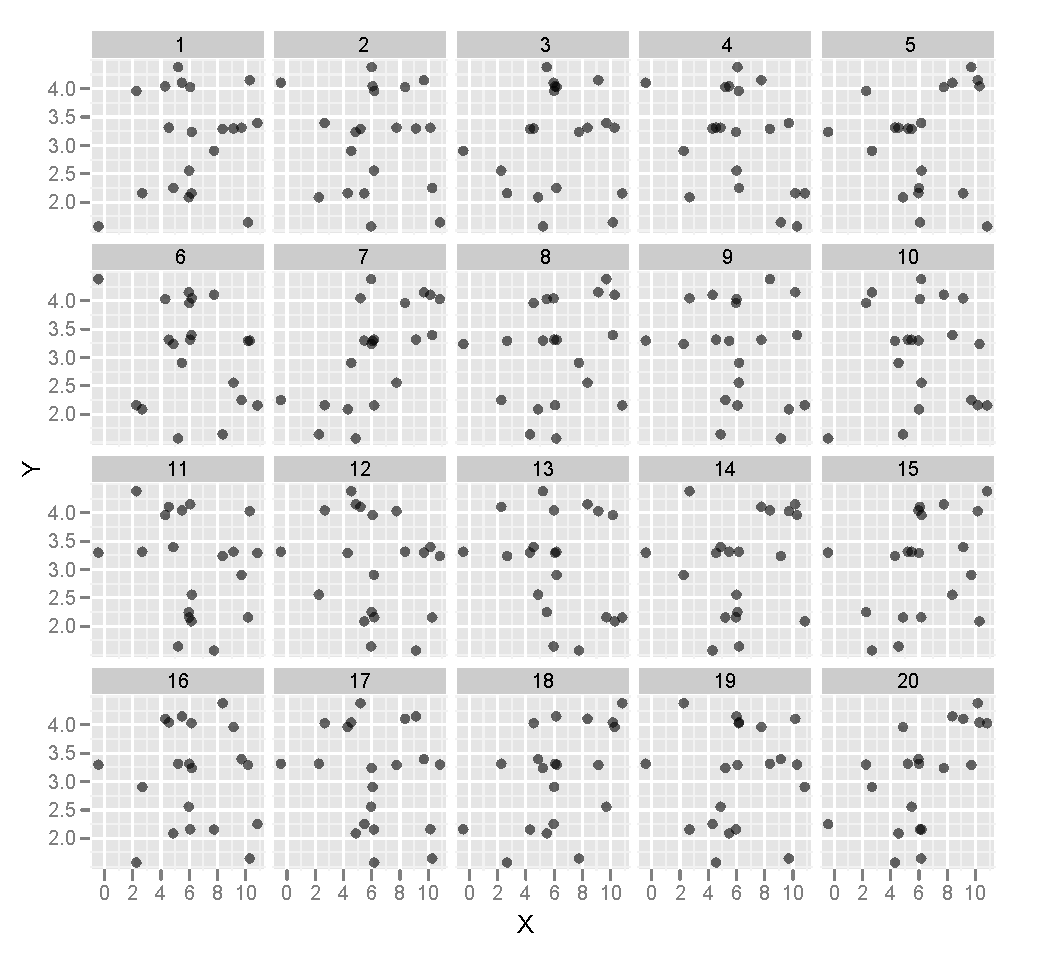
\includegraphics[scale=0.41]{sca2.pdf}
\label{sca_1}
}
\subfigure[]{
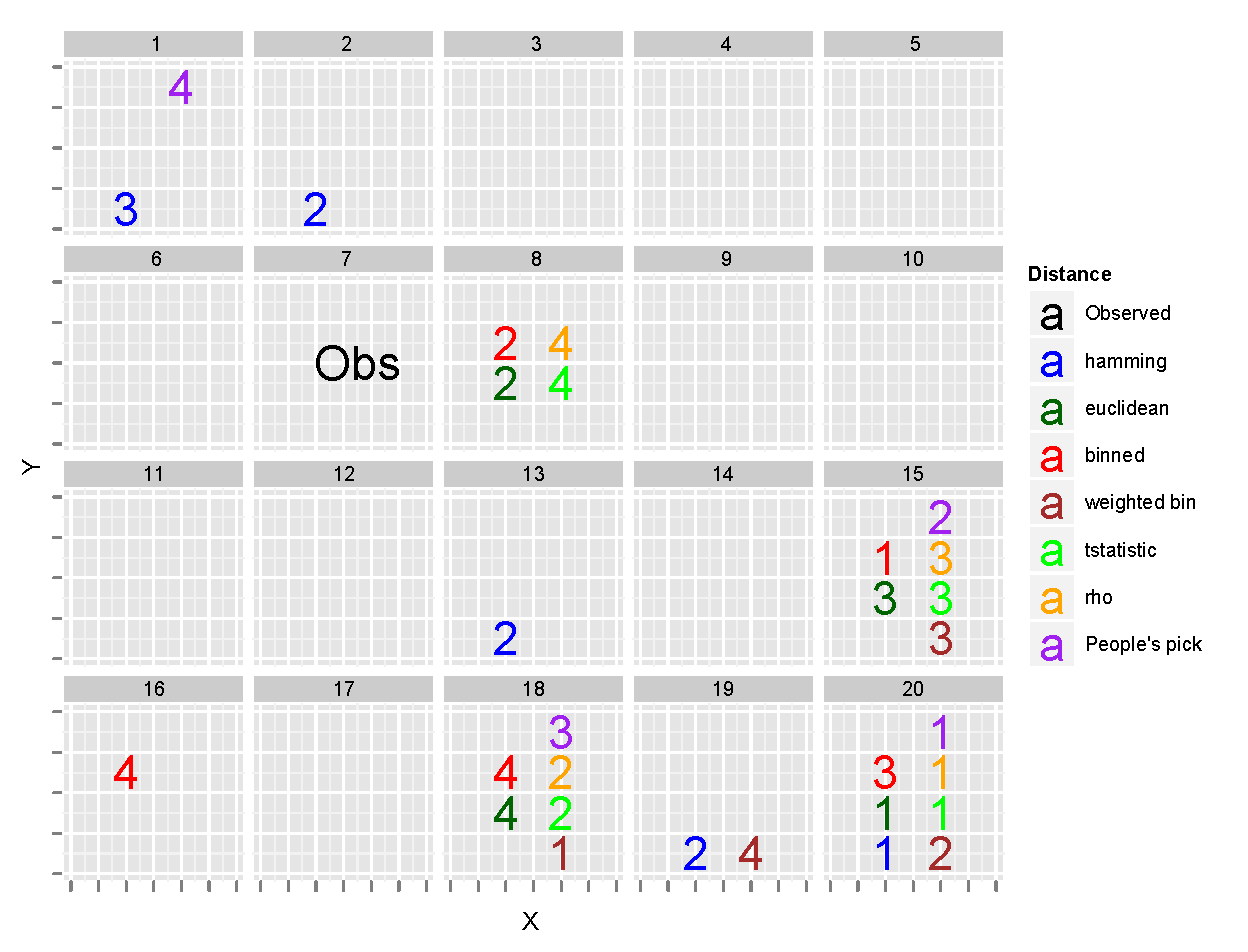
\includegraphics[scale=0.41]{dist_lineup_final.pdf}
\label{sca_2}
}
\label{sca_lineup}
	\vspace{-.1in}
\caption[Optional caption for list of figures]{(a) Lineup Plot ($m$ = 20) for testing whether there exists a positive association between $X$ and $Y$. The 19 null plots are obtained by permuting $Y$ of the observed data while keeping $X$ fixed. Can you identify the observed plot?  (b) The chart on the right gives an overview of the closest plots according to all distance measures. The People's pick is discussed in more detail in Section~\ref{user.distance}. }
%{Caption of subfigures \subref{fig:subfig1}, \subref{fig:subfig2} and \subref{fig:subfig3}}
\end{figure*}


%\blue{\section{A user defined distance}\label{user.distance}
%In order to match the distance measures above to what we actually `see' in a plot, we conducted an experiment asking an audience to judge closeness of null plots to the actual data plot.
%Each participant was given 5 lineup plots similar to figure \ref{fig:subfig1}. For each lineup, the participant was asked which of the plots exhibited the strongest positive association between the variables. In a next step, the actual data plot was identified and participants were asked to identify the plots that most closely matched the data plot. 
%
%For this study, we had a set of 15 participants evaluating 5 line-ups (of 20 plots) with respect to similarity of nullplots to the actual data chart. The number of `close' charts was not specified -- in the study we observed between 1 and 5 responses, with most participants picking 2-3 close charts.
%
%Based on these ranks we define an {\it audience distance} as follows:
%
%\red{Describe how the data looks like. Then describe how we can use the data to get a user defined 'closeness' or distance.}
%}


\section{Example, using Scatterplots} \label{sec:asso}

Consider a dataset with two continuous variables $X$ and $Y$. 
%Let us assume that one variable is the explanatory or independent variable ($X$) and the other variable is the response or dependent variable ($Y$). 
We are interested in whether there exists a significant positive association between the two variables. To test this we generate a scatterplot of the two variables. If there exists a positive association between the two variables, their values should be close to a line in a scatterplot. \\ \\%the scatterplot shows that the points fall close to the diagonal line in the positive direction. \\ \\
Assuming independence between the variables, we generate null plots by permuting the response variable i.e. $Y$ while keeping the explanatory variable i.e. $X$ fixed. 
The test statistic, the plot containing the observed data, is placed randomly among 19 null plots as shown in the line up in  Figure \ref{sca_1}. If the test statistic is identifiable, the null hypothesis is rejected with a $p$-value of at most 0.05.\\

%A lineup including the test statistic is shown in Figure \ref{fig:subfig1}.  The 19 null plots are generated by permuting the response variable i.e. $Y$ while keeping the explanatory variable i.e. $X$ fixed. The test statistic, the plot containing the observed data, is placed randomly among these null plots. If the test statistic is identifiable, the null hypothesis is rejected with a $p$-value of at most 0.05. \\ 

%\begin{figure*}[hbt]
%%\begin{figurehere}
%   \centering
%       \scalebox{0.45}{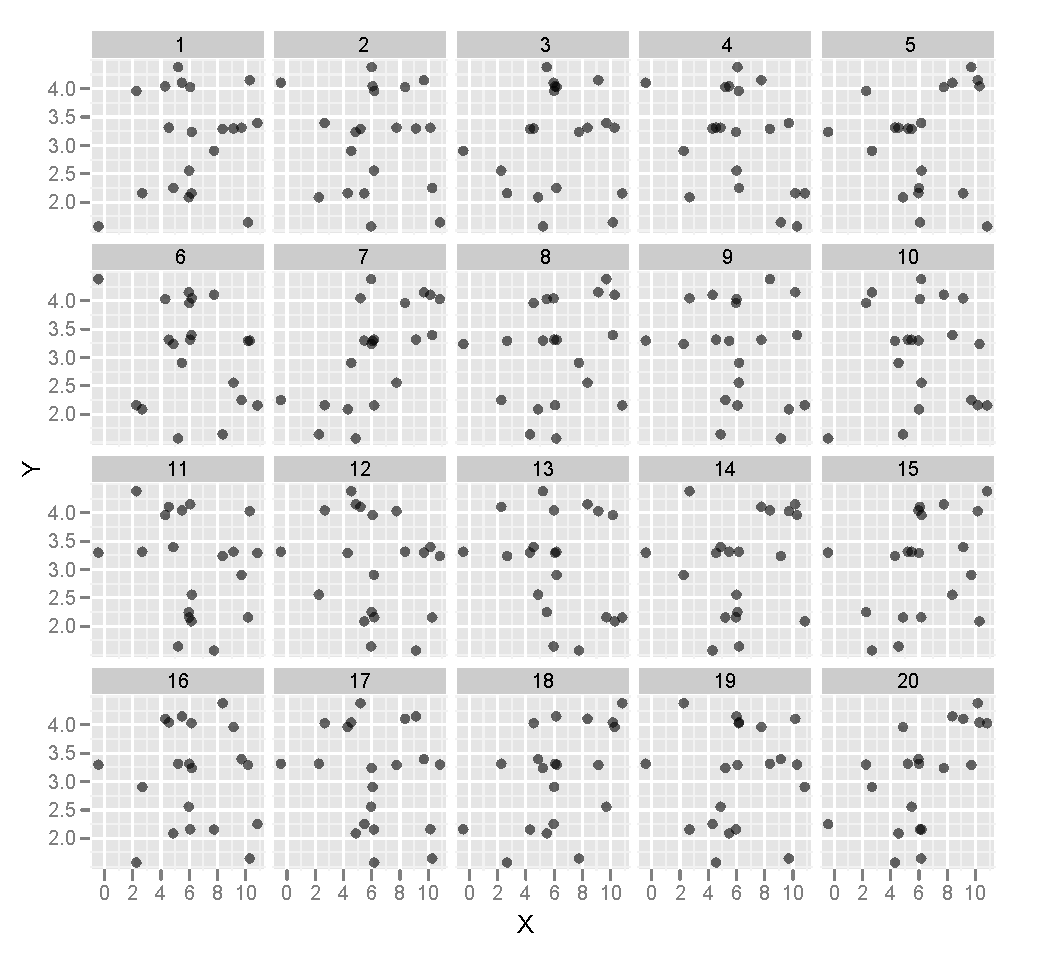
\includegraphics{sca2.pdf}}
%	\scalebox{0.45}{\includegraphics{dist_lineup_6.pdf}}
%
%       \caption{Lineup Plot (m = 20) for testing whether there exists a positive association between $X$ and $Y$. The 19 null plots are obtained by permuting $Y$ of the observed data while keeping $X$ fixed. Can you identify the observed plot?}
%       \label{sca_lineup}
%\end{figure*}

For each of the null plots in the lineup, we compute all of the distances to the observed plot.
The distances between the observed plot and 19 null plots are calculated. 
%Since both the variables are continuous, we can calculate all the distances except the Wilcoxon Rank Sum Test which requires grouping in the data which is absent in this case. 
%\red{there's a lot of overlap between this section and the discussion of the distances. You could shorten things here.}\green{I tried to make this short but I could not do much about this.}
%The Hamming distance is calculated on the basis of only the permutations of the variable $Y$ and the actual values of the variable are not being used. The $t$-statistic is calculated on the basis of the correlation coefficient between the unchanged $X$ and the permuted $Y$ for each of the 19 null plots. 
For calculating the binned and the weighted binned distances, we consider a 10 $\times$ 10 grid ($p$ = $q$ = 10) for a total of 100 cells. \\

In order to  quantify  these distances, we generate empirical distributions based on 10,000 permutations of $Y$ and estimate corresponding $p$ values as lower tail percentages. 
%We also calculated the percentile values for each of the null plots for each of the distances. For calculating the percentile values, we generated 10,000 permutations of $Y$ and calculated the different distance measures based on these permutations to obtain the empirical distribution of each of the distance measures.
 Figure \ref{emp_wbdist} gives  the empirical distribution of the weighted binned distance for our line-up based on a 10 $\times$ 10 grid. \\

\begin{figure}[hbtp]
%\begin{figurehere}
   \centering
       \scalebox{0.4}{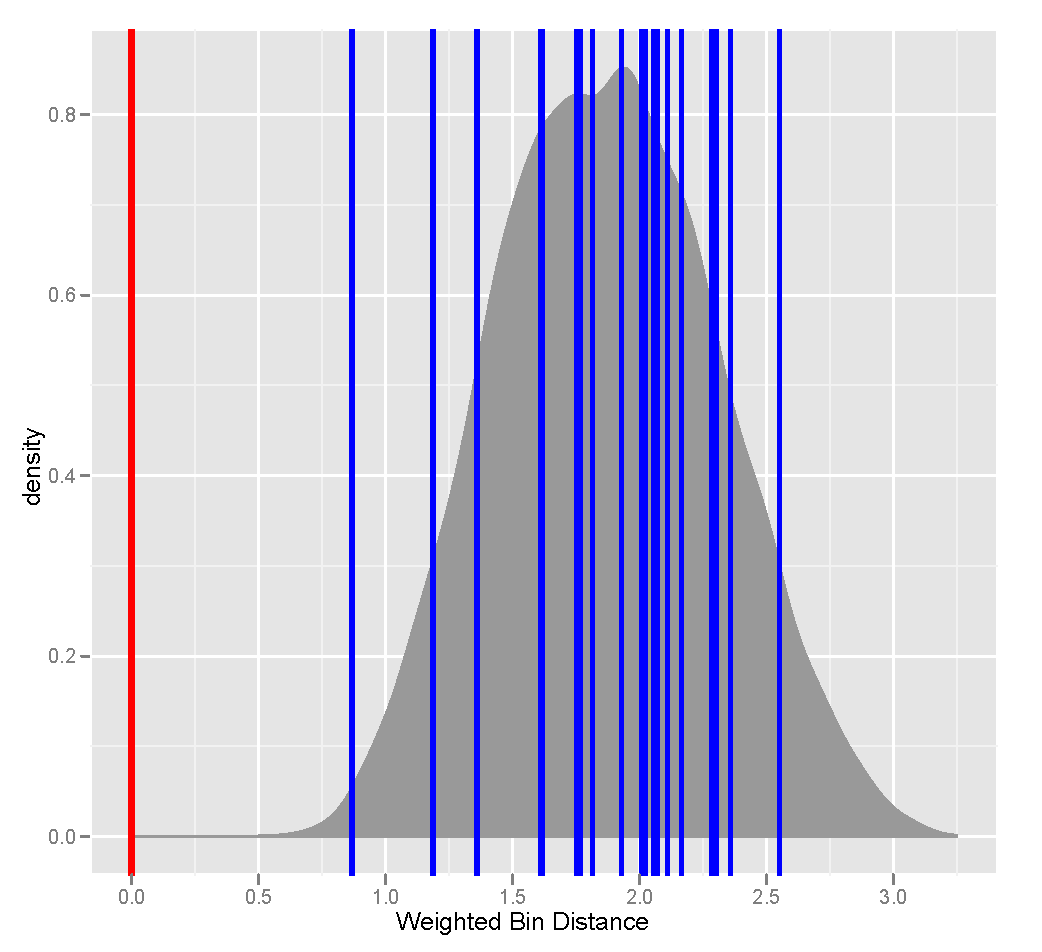
\includegraphics{emp_wbdist3.pdf}}
	\vspace{-.1in}
       \caption{Density plot of Weighted Binned Distance from observed data plot.  The vertical red line (at $x=0$)  corresponds to the observed data plot. The blue vertical lines show the weighted bin distances between the observed plot to all the other 19 null plots in the lineup.  }
       \label{emp_wbdist}
\end{figure}

%\red{Explain, why this score helps us in the comparison - when is the score high, when is it low?} 
One way to measure the `difficulty' of spotting the observed data plot in the line-up is given by how far away the red line for the observed plot is from the blue lines of the null plots. For that, 
%We are interested in how close a null plot is to the observed plot. Moreover we want to compare multiple lineups generated from the same observed data. So 
we calculate a $z$-score value for each of the distance measures by subtracting the mean of the empirical distribution from the distance %measures from the distance measures obtained for each of the 20 plots 
and dividing it by the (empirical) standard deviation. 
%of the empirical distribution of the distance measures. 
So, for the Hamming distances,  the $z$-score for the $k$-th plot in the lineup is obtained as 
\[
z_k = \frac{h_k - \mu_H}{\sigma_H}
\]
where $h_k$ gives the realized hamming distances for the $k$-th plot in the lineup where $k = 1, \dots, 20$ and $\mu_H$ and $\sigma_H$ gives the mean and the standard deviation of the empirical distribution of the hamming distances, respectively. 

%if $H$ denotes the random variable following the empirical distribution of the hamming distances and , then


On the basis of the $z$-scores, we can compare the null plots to the observed plot. Here, $\sigma_H$ acts as a ruler which tells us how far each of these 20 plots is from $\mu_H$. Since all of the distance measures are 0 %the hamming , euclidean, binned and weighted bin distance measures are 0 
for the observed plot, the $z$-scores for the observed plot for the above measures will simply be $-\mu_H/\sigma_H$. For the 19 null plots, a low $z$-score indicates that the null plot is close to the observed plot and a high $z$-score indicates that the null plot is far from the observed plot on the basis of the corresponding distance measure. 

Table \ref{sca_table} shows $z$-scores and percentile values of all distance measures for the lineup of Figure~\ref{sca_1}. %}obtained based on the the six different distance measures. 
For each distance metric, we show all results within a 25\% percentile of the empirical distribution of the distance from the actual data plot, ordered from most similar to least similar. 
Figure~\ref{sca_2} gives a graphical representation of the table. We can see that most distance measures agree on plot 20 as most similar  to the observed data plot, followed by plots 15 and 18.

%We order the 19 null plots based on the lowest $z$-scores and the percentile values. Since the six distance measures have different $z$-scores, we have six different sets of ordered null plots. Table \ref{sca_table} shows only the plots whose distance measure is less than the first quartile of the distances obtained for the null plots. 
% \red{Put in more description for the table: how is the sorting done, why do you only show some plots. }
%\red{paraphrase this formula in words. If you want to use a formula, don't use words - it looks unprofessional.}
%\red{What is the conclusion from the table?} \green{I need to write the conclusions but should I explain for all the distance measures or one particular example.}

\begin{table*}[hbt]
	\vspace{-.1in}
\caption{Percentile values and $z$ scores of closest distances from the observed data plot in the lineup of Figure~\ref{sca_1}. Rows are ordered according to minimal distance from the observed data plot within each of the distance measures. Plot 20 is close to the observed data plot for all  of the distances.}
%Table showing the different distance matrices and the percentile values of each distance 
%\red{also explain the ordering - and don't report the numbers at this precision.} \green{I am not sure what precision I should use.}
%
\centering  % centering table
\begin{tabular}{l r rrrr r rrr}  % creating 10 columns
\hline                       % inserting double-line
Distance & Plot No &\multicolumn{4}{c}{$z$-score} & &\multicolumn{3}{c}{Percentile Value} \\ [0.5ex]   
 \cline{1-1}\cline{3-6}\cline{8-10}
 & & Hamming & Euclidean & Binned & Wgtd Bin & & t statistic & $\rho$ & People's   \\     [0.5ex]
\hline
%% Entering 4th row
Hamming  & 20 & $\bf -2$ & $-1.7$ & $-1.7$ & $-1.6$ & & 0.3 & 0.8 & 45.8 \\[-0.5ex]
 & 2 & $\bf -1$ & 0.3 & $-0.4$ & $-1.0$ & & 62.2 & 38.4 & 0.0\\[-0.5ex]
 & 13 & $\bf  -1$ & 0.3 & 0.7 & 1.1 & & 85.6 & 88.9 & 0.0 \\[-0.5ex]
& 19 & $\bf -1$ & $0.6$ & $-1.3$ & $-1.2$ &  & $36.8$ & $22.5$ & 0.0 \\[-0.5ex]
 & 1 & $\bf 0$ & $-1.2$ & 0.7 & $-0.6$ & & 22.3 & 33.8 & 8.3 \\[1ex]

%%% Entering 4th row
Euclidean  & 20 & $-2$ & $\bf -1.8$ & $-1.7$ & $-1.6$ & & $0.3$ & $0.8$  & 45.8 \\[-0.5ex]
		 & 8 & $ 1$ & $\bf -1.7$ & $-2.2$ & $-1.0$ & & $18.1$ & $10.4$ & 0.0 \\[-0.5ex]
 		& 15 & $1$ & $\bf -1.7$ & $-2.7$ & $ -1.4$ & & $7.7$ & $4.5$ & 33.3\\[-0.5ex]
 		& 18 & $1$ & $\bf -1.4$ & $-1.3$ & $ -2.0$ & & $1.9$ & $2.3$ & 12.5\\[1ex]

%%% Entering 4th row
Binned  & 15 & $1$ & $-1.7$ & $\bf -2.7$ & $ -1.4$ & & $7.7$ & $4.5$ & 33.3\\[-0.5ex]
	    & 8 & $ 1$ & $-1.7$ & $\bf -2.2$ & $-1.0$ & & $18.1$ & $10.4$ & 0 \\[-0.5ex]
	   & 20 & $-2$ & $-1.8$ & $\bf -1.7$ & $ -1.6$ & & $0.3$ & $0.8$ & 45.8 \\[-0.5ex]
 		& 16  & $1$ & $-0.9$ & $\bf -1.3$ & $-0.2$ & & 55.1 & 56.1 & 0\\[-0.5ex]
		& 18 & $1$ & $-1.4$ & $\bf -1.3$ & $\bf -2.0$ & & $1.9$ & $2.3$ & 12.5\\[1ex]

%%% Entering 4th row
Weighted Bin & 18 & $1$ & $-1.4$ & $-1.3$ & $\bf -2.0$ & & $1.9$ & $2.3$ & 12.5 \\[-0.5ex]
		 & 20 & $-2$ & $-1.8$ & $-1.7$ & $\bf -1.6$ & & $0.3$ & $0.8$ & 45.8 \\[-0.5ex]
 		& 15 & $1$ & $-1.7$ & $-2.7$ & $\bf -1.4$ & & $7.7$ & $4.5$ & 33.3 \\[-0.5ex]
 		& 19 & $-1$ & $0.6$ & $-1.3$ & $\bf -1.2$ & & $36.8$ & $22.5$ & 0\\[1ex]

%%% Entering 4th row
t statistic  & 20 & $-2$ & $-1.8$ & $-1.7$ & $ -1.6$ & & $\bf 0.3$ & $0.8$ & 45.8 \\[-0.5ex]
		  & 18 & $1$ & $-1.4$ & $-1.3$ & $ -2.0$ & & $\bf 1.9$ & $2.3$ & 12.5\\[-0.5ex]
		& 15 & $1$ & $-1.7$ & $-2.7$ & $ -1.4$ & & $\bf 7.7$ & $4.5$ & 33.3 \\[-0.5ex]
 		 & 8 & $ 1$ & $-1.7$ & $-2.2$ & $-1.0$ & & $\bf18.1$ & $10.4$ & 0 \\[1ex]

%%% Entering 4th row
Spearman's $\rho$  & 20 & $-2$ & $-1.8$ & $-1.7$ & $ -1.6$ & & $0.3$ & $\bf 0.8$ & 45.8 \\[-0.5ex]
		   & 18 & $1$ & $-1.4$ & $-1.3$ & $ -2.0$ & & $1.9$ & $\bf 2.3$ & 12.5 \\[-0.5ex]
		 & 15 & $1$ & $-1.7$ & $-2.7$ & $ -1.4$ & & $7.7$ & $\bf 4.5$ & 33.3 \\[-0.5ex]
 		 & 8 & $ 1$ & $-1.7$ & $-2.2$ & $-1.0$ & & $18.1$ & $\bf 10.4$ & 0\\[1ex]

People's pick  	& 20 & $-2$ & $-1.8$ & $-1.7$ & $ -1.6$ & & $0.3$ & $0.8$ & $\bf 45.8$ \\[-0.5ex]  
		 & 15 & $1$ & $-1.7$ & $-2.7$ & $ -1.4$ & & $7.7$ & $4.5$ & $\bf 33.3$ \\[-0.5ex]
		  & 18 & $1$ & $-1.4$ & $-1.3$ & $ -2.0$ & & $1.9$ & $2.3$ & $\bf 12.5$ \\[1ex]

\hline
Actual & 7  & $-19$ & $-8.5$ & $-9.9$ & $-4.1$ & & 0.1 & 0.2 & 93.3\\[1ex]
\hline
\end{tabular}
\label{sca_table}
\end{table*}


%\begin{table*}[hbt]
%\caption{Table showing the different distance matrices and the percentile values of each distance \red{also explain the ordering - and don't report the numbers at this precision.}}
%\centering  % centering table
%\begin{tabular}{l r rrrr rr}  % creating 10 columns
%\hline\hline                       % inserting double-line
%Distance & PlotNo &\multicolumn{4}{c}{$z$-score} &\multicolumn{2}{c}{Percentile Value}  \\ [0.5ex]   
%\hline  \hline
% & & Hamming & Euclidean & Binned & Weighted Bin & t statistic & Spearman's $\rho$   \\     [0.5ex]
%\hline
%%% Entering 4th row
%Hamming  & 11 & $-3.987$ & $0.577$ & $-1.592$ & $1.134$ & 57.55 & 55.35  \\[-0.5ex]
% & 6  & $-1.993$ & $-0.961$ & $-0.817$ & $-1.178$ & 37.14 & 51.32\\[-0.5ex]
% & 19  & $-1.993$ & $-0.331$ & $-0.101$ & $-0.588$ &  45.04 & 23.54\\[-0.5ex]
% & 20  & $-1.993$ & $0.439$ & $-0.101$ & $-0.125$ & 48.59 & 58.92\\[1ex]
%\hline
%%%% Entering 4th row
%Euclidean  & 18 & $0.997$ & $-1.416$ & $-0.817$ & $-0.603$ & 63.77 & 61.26  \\[-0.5ex]
%		 & 2  & $0.997$ & $-1.409$ & $0.570$ & $-0.233$ & 49.59 & 47.80\\[-0.5ex]
% 		& 6  & $-1.993$ & $-0.961$ & $-0.817$ & $-1.178$ & 37.14 & 51.32\\[-0.5ex]
% 		& 8  & $0.000$ & $-0.712$ & $-0.817$ & $-2.319$ & 7.52 & 13.01\\[1ex]
%\hline
%%%% Entering 4th row
%Binned  & 11 & $-3.987$ & $0.577$ & $-1.592$ & $1.134$ & 57.55 & 55.35  \\[-0.5ex]
%		 & 12  & $-0.997$ & $0.495$ & $-1.592$ & $-1.583$ & 21.17 & 14.97\\[-0.5ex]
%		& 14  & $0.997$ & $0.592$ & $-1.196$ & $0.688$ & 81.46 & 84.51 \\[-0.5ex]
% 		& 6  & $-1.993$ & $-0.961$ & $-0.817$ & $-1.178$ & 37.14 & 51.32\\[-0.5ex]
% 		& 8  & $0.000$ & $-0.712$ & $-0.817$ & $-2.319$ & 7.52 & 13.01\\[-0.5ex]
%		& 13  & $0.000$ & $1.080$ & $-0.817$ & $-0.272$ & 9.64 & 17.96\\[-0.5ex]
%		& 18 & $0.997$ & $-1.416$ & $-0.817$ & $-0.603$ & 63.77 & 61.26  \\[1ex]
%\hline
%%%% Entering 4th row
%Weighted Bin & 8  & $0.000$ & $-0.712$ & $-0.817$ & $-2.319$ & 7.52 & 13.01  \\[-0.5ex]
%		 & 12  & $-0.997$ & $0.495$ & $-1.592$ & $-1.583$ & 21.17 & 14.97\\[-0.5ex]
% 		& 6  & $-1.993$ & $-0.961$ & $-0.817$ & $-1.178$ & 37.14 & 51.32\\[-0.5ex]
% 		& 18 & $0.997$ & $-1.416$ & $-0.817$ & $-0.603$ & 63.77 & 61.26\\[1ex]
%\hline
%%%% Entering 4th row
%t statistic & 8  & $0.000$ & $-0.712$ & $-0.817$ & $-2.319$ & 7.52 & 13.01  \\[-0.5ex]
%		  & 13  & $0.000$ & $1.080$ & $-0.817$ & $-0.272$ & 9.64 & 17.96\\[-0.5ex]
%		 & 12  & $-0.997$ & $0.495$ & $-1.592$ & $-1.583$ & 21.17 & 14.97\\[-0.5ex]
% 		& 17 & $0.000$ & $0.433$ & $-0.101$ & $0.355$ & 25.53 & 13.13\\[1ex]
%\hline
%%%% Entering 4th row
%Spearman's $\rho$ & 8  & $0.000$ & $-0.712$ & $-0.817$ & $-2.319$ & 7.52 & 13.01  \\[-0.5ex]
%		 & 17 & $0.000$ & $0.433$ & $-0.101$ & $0.355$ & 25.53 & 13.13\\[-0.5ex]
% 		 & 12  & $-0.997$ & $0.495$ & $-1.592$ & $-1.583$ & 21.17 & 14.97\\[-0.5ex]
% 		& 13  & $0.000$ & $1.080$ & $-0.817$ & $-0.272$ & 9.64 & 17.96\\[1ex]
%\hline
%Actual & 7  & $-18.939$ & $-8.428$ & $-10.481$ & $-4.332$ & & \\[1ex]
%\hline
%\end{tabular}
%\label{sca_table}
%\end{table*}


\section{Results}\label{results}
%%\red{this results section refers to the dotplots, I think - this needs to be fixed.} \green{I changed this part, but most of the things that I wanted to write has gone to the previous section.}
The experiment is conducted to study the ability of human observers to detect the positive association between two continuous variables. Data is simulated with the sample size $n = 20$ and $n=30$. The continuous variables ($X$,$Y$) are generated from a Bivariate Normal distribution with $\mu_X = 6$, $\mu_Y = 3$, $\sigma_X = 4$, $\sigma_Y = 1$, $\rho_{XY} = \rho$ where $\rho$ is generated from a Uni(0.2, 0.7). Five replicates of the above combination are generated (four with $n =20$ and one with $n=30$). These produced five different ``observed data sets''. The null plots for the lineups was generated from each of the data sets. \\

Figure \ref{dist_1} and Figure \ref{dist_2} gives scatterplots of the People's pick against the z-scores and the percentiles for the distance measures. $R^2$ gives a measure of the correlation between People's pick and the distance measures. The median $R^2$ from the 5 lineups indicates that Spearman's $\rho$ worked best followed by t-statistic and weighted bin.

%\begin{table}[hbt]
%\caption{Table showing the $R^2$ values for each distance measures.}
%\centering  % centering table
%\begin{tabular}{l l }  % creating 10 columns
%Distance & $R^2$\\
%\hline
%Hamming & 0.06 \\
%Euclidean & 0.02 \\
%Binned & 0.002 \\
%Weighted Bin & 0.23 \\
% tstatistic & 0.34 \\
% $\rho$ & 0.29 \\
%\hline
%\end{tabular}
%\label{rsquare}
%\end{table}

%
%\begin{figure}[hbt]
%%\begin{figurehere}
%   \centering
%       \scalebox{0.5}{\includegraphics{per_res_vs_dist.pdf}}
%       \caption{Plot showing the different distance measures by the different plots for the dotplots.}
%%\green{Dr. Cook wanted me to change this plot but I do not know what to do with this.}}
%       \label{dot_summary}
%\end{figure}

%\begin{figure*}[hbt]
%%\begin{figurehere}
%   \centering
%       \scalebox{0.45}{\includegraphics{plotvsdist_dot.pdf}}
%       \caption{Plot showing the different distance measures by the different plots for the dotplots.}
%       \label{dot_summary}
%\end{figure*}
%
%\begin{figure}[hbt]
%%\begin{figurehere}
%   \centering
%       \scalebox{0.45}{\includegraphics{plotvsdist_sca.pdf}}
%       \caption{Plot showing the different distance measures by the different plots for the scatterplots.}
%       \label{fig:test_category}
%\end{figure}

\section{Conclusions} \label{sec:conclusions}
%\green{This section has to be written down}
The purpose of this paper has been to take a closer look at the null plots that comes up in a lineup along with the observed plot. We do that with the help of some distance measures that gives us the measure of closeness of the null plots to the observed plot. For this experiment the closeness was measured in case of a scatterplot. Future experiments will be conducted to measure closeness among other types of plots which may use of other distance measures.

%The purpose of this paper has been to examine the effectiveness of visual inference methods in direct comparison to existing inference methods. We need to be clear that this is not the purpose of visual inference generally: visual methods should not be seen as competitors to traditional inference.  The purpose here, is to  establish properties and  efficacy of visual testing procedures in order to use them in situations where traditional tests cannot be used. For this experiment the effect of $\beta_2$ was examined using side-by-side boxplots. Future experiments will be conducted to compare other regression parameters as described in Table \ref{tbl:stat_multiple} and assess sensitivity of power to modeling conditions.

\begin{figure*}[htbp]
\centering
\subfigure[]{
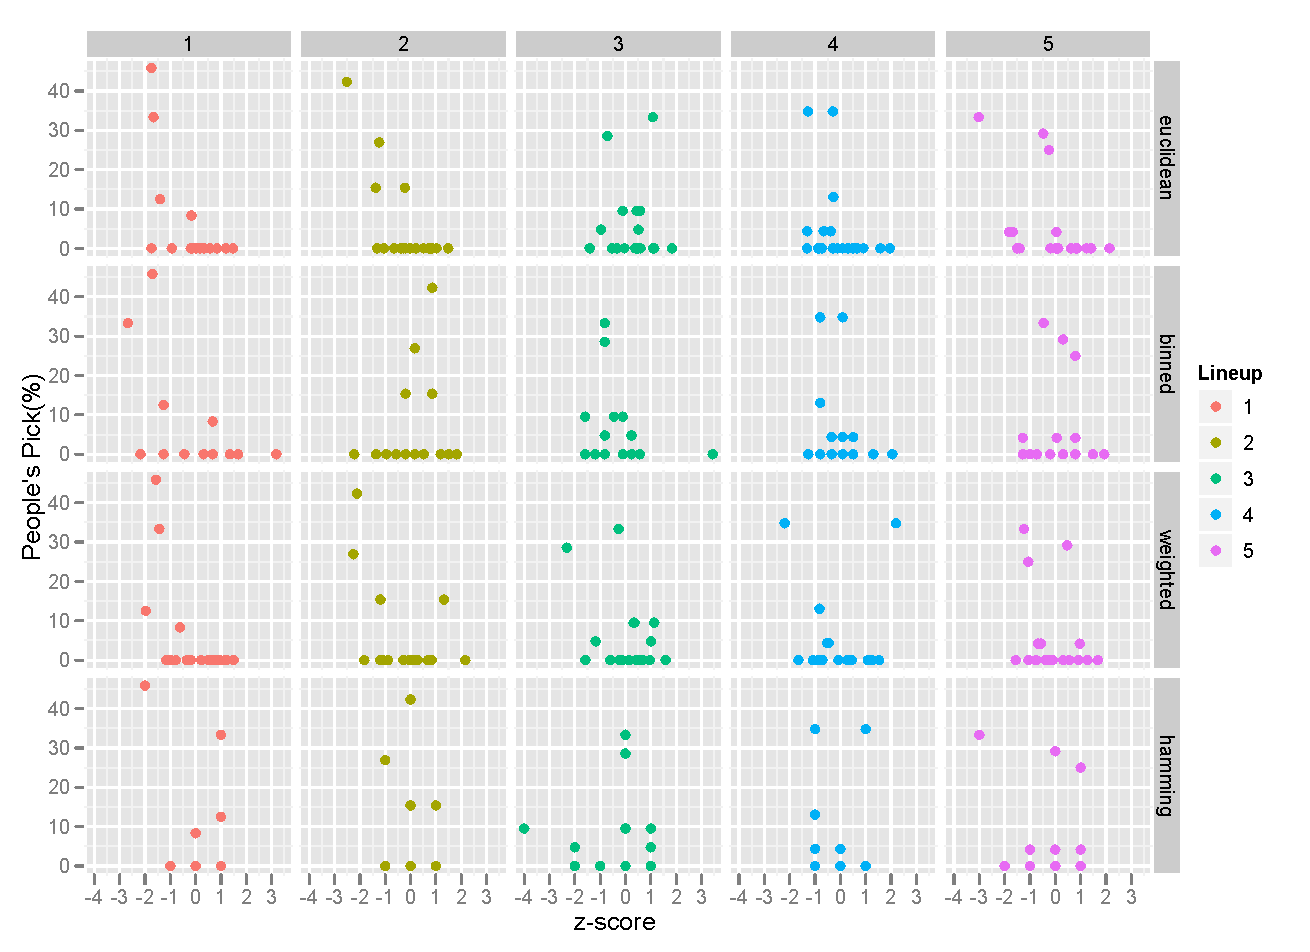
\includegraphics[scale=0.7]{dist_vs_zscore.pdf}
\label{dist_1}
}
\subfigure[]{
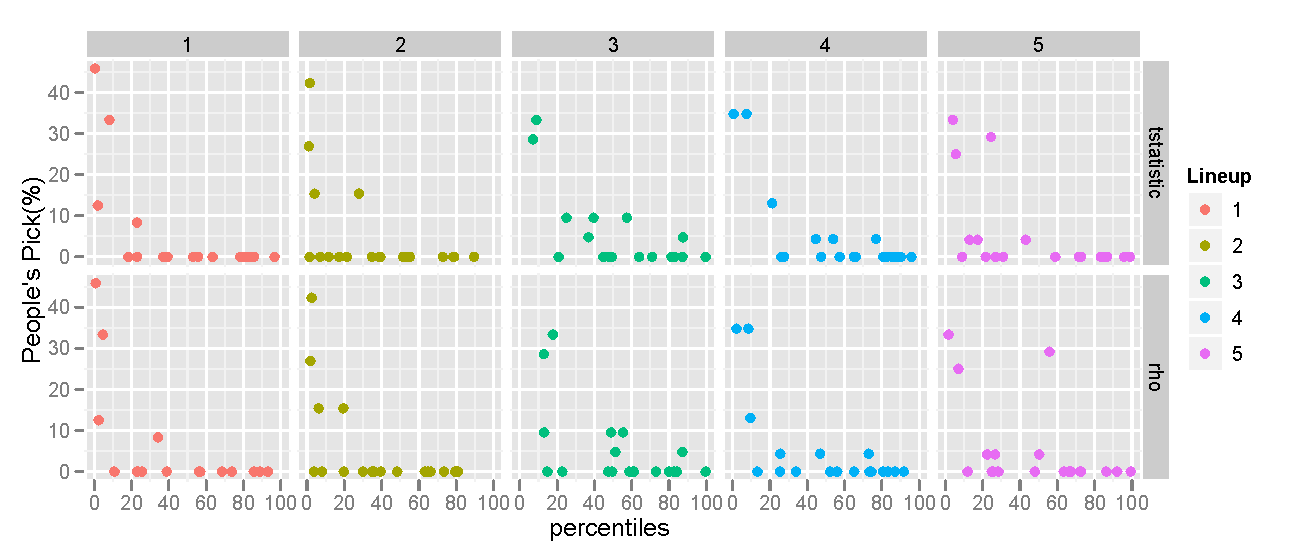
\includegraphics[scale=0.7]{dist_vs_percentile.pdf}
\label{dist_2}
}
\label{dist_z_perc}
	\vspace{-.1in}
\caption[Optional caption for list of figures]{(a) Scatterplot of the People's pick against the z-scores for each distance measure colored by the lineups. (b) Scatterplot of the People's pick against the percentiles for t-statistic and Spearman's $\rho$ colored by the lineups. }
%{Caption of subfigures \subref{fig:subfig1}, \subref{fig:subfig2} and \subref{fig:subfig3}}
\end{figure*}

%\newpage

     
        
%\begin{figure}[hbtp]
%%\begin{figurehere}
%   \centering
%       \scalebox{0.4}{\includegraphics{data4_10_10_10_1.pdf}}
%       \caption{Dataset 4}
%	\vspace{-.1in}
%\end{figure}        
% 
\paragraph{Acknowledgement:}

This work was funded by National Science Foundation grant DMS 1007697. All plots are done with the {\tt ggplot2} \citep{hadley:2009} package in R.
